\subsection{Parameter Identification}

\begin{figure}[h]
    \centering
    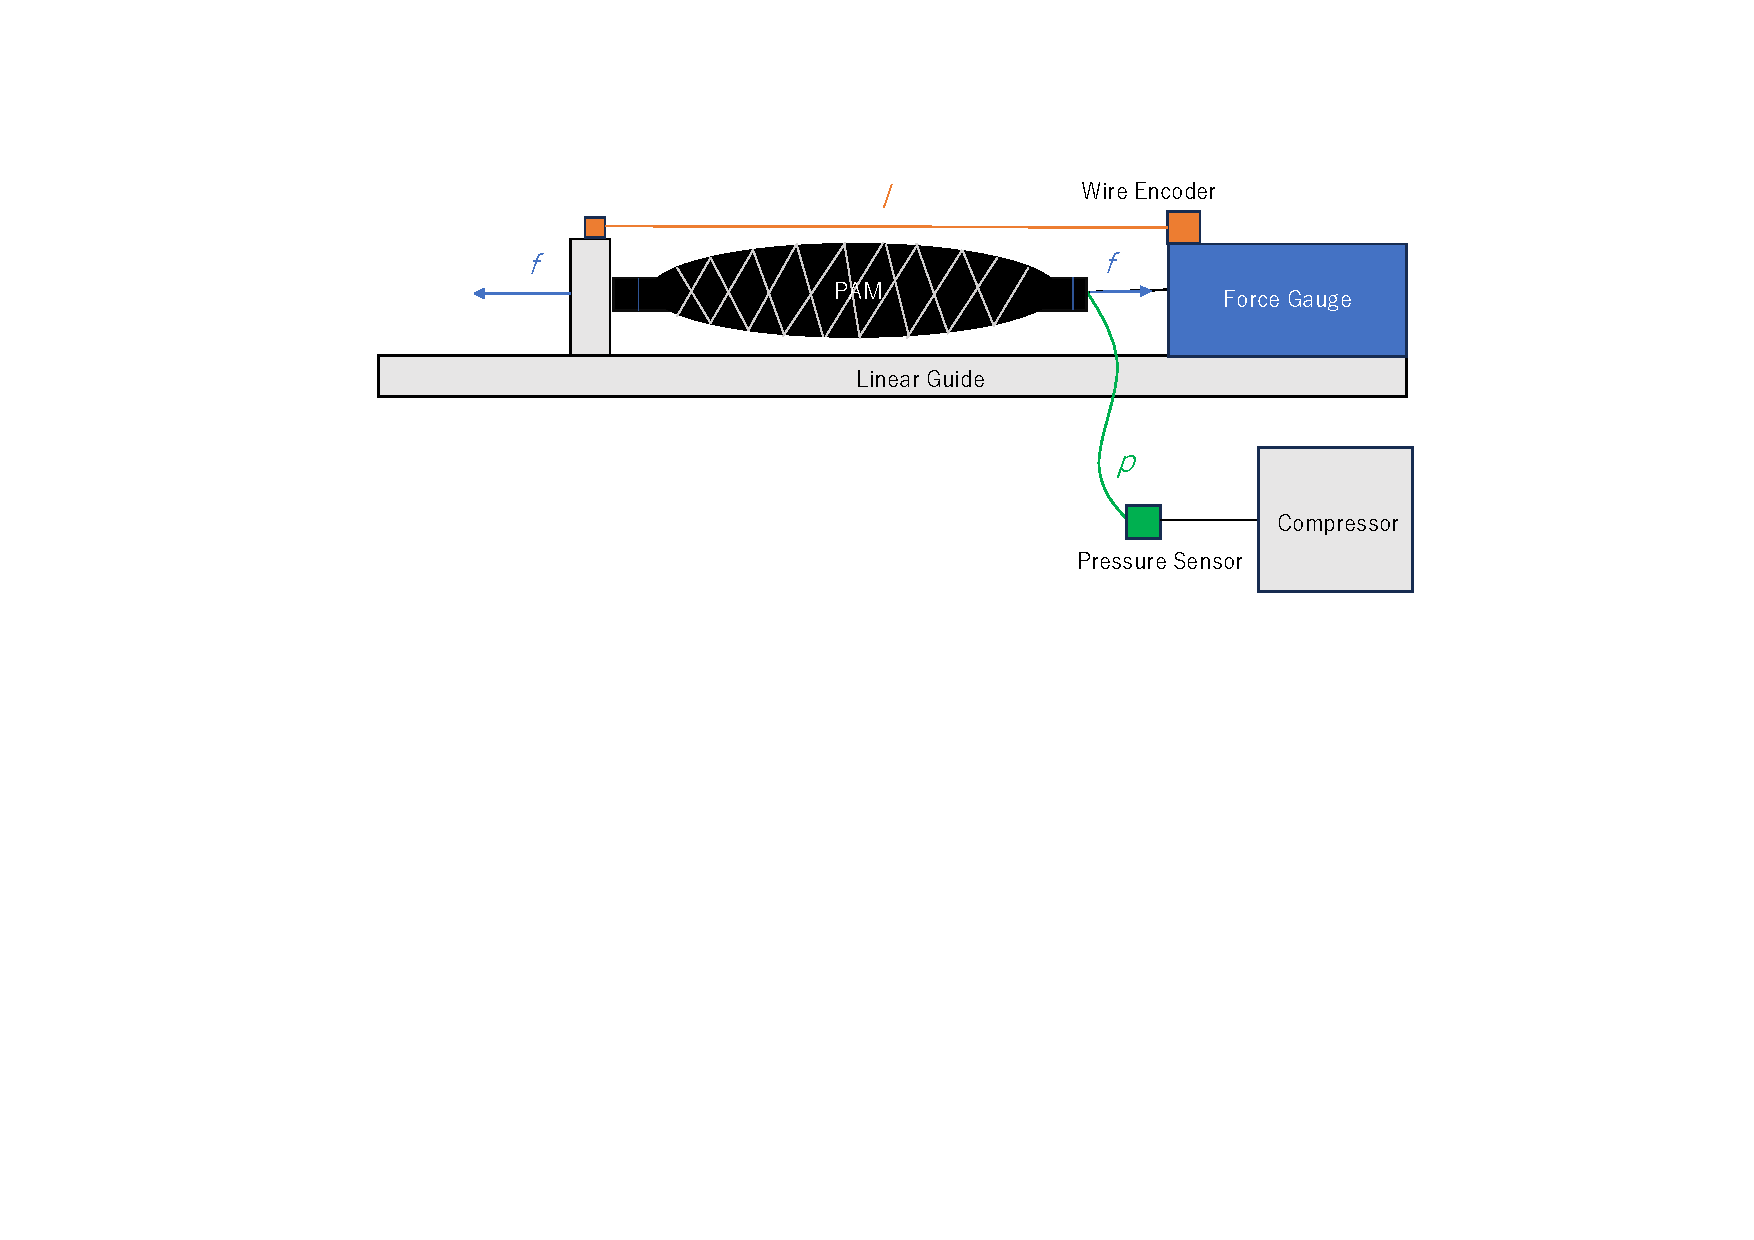
\includegraphics[width=\columnwidth]{fig/static_experiment.pdf}
    \caption{Outline Diagram of Static Loading Experiment}
    \label{fig:static_equipment}
 \end{figure}

Fig. \ref{fig:static_equipment} is an outline diagram of the static loading experiment to identify the parameters $m$, $h$, and $a_i$ .
Table \ref{tab:PAM} shows the shapes and materials of the used four PAMs (A,B,C,D).
The experimental procedure was as follows.
First, the pressure $p$ was adjusted to a constant level.
Taking into account the strength of the materials, the pressure of PAM-A, PAM-B, or PAM-C was adjusted to $0.4\si{MPa}$, $0.5\si{MPa}$, $0.6\si{MPa}$, $0.7\si{MPa}$ or $0.8\si{MPa}$, while the pressure of PAM-D was $0.2\si{MPa}$, $0.3\si{MPa}$, $0.4\si{MPa}$, $0.5\si{MPa}$, or $0.6\si{MPa}$.
Next, the PAM was gradually stretched from the natural length by y $2.5\si{mm}$ increments and the deformation $d$, the force $f$, and the pressure $p$ were measured at each point.
Each value was stabilized by waiting for at least 2 seconds after deformation.
Once $d$ reached its maximum value predetermined based on each PAM's strength, it was contracted to the natural length $l_n$ by  $2.5\si{mm}$ decrements, and $d$, $p$, and $f$ were measured again at each point.
Finally, the parameters $m$, $h$, and $a_i$ were calculated by the least squares method.
The pressure sensor used was PSE540(SMC Co.), the linear encoder was DS-025(MUTOH INDUSTRIES Co. Ltd.), and the force gauge was FGP-5(Nidec Co.).

\begin{table}[h]
    \centering
    \caption{Characteristics of Experimented PAMs}
    \begin{tabular}{c|ccccc}
        \hline
        PAM & Length [$\si{mm}$] & Diameter [$\si{mm}$] & bladder Material\\
        \hline \hline
        A & 216 & 19.9 &  Rubber \\
        B &211  & 13.4 &  Rubber \\
        C & 141 & 13.4 &  Rubber \\
        D & 212 & 19.0 & Silicon \\
        Agonist & 180 & 16.0 & Rubber \\
        Antagonist & 180 & 16.1 & Rubber \\
        \hline
    \end{tabular}
\label{tab:PAM}
\end{table}


\subsection{Error Evaluation}
We dynamically estimated the length of the four different PAMs to verify the general applicability of the model.
The jig holding the left end of the PAM in Fig. \ref{fig:static_equipment} was removed and a pulley was installed in its place. A proportional control valve was installed between the pressure sensor and the compressor.
The experiment procedure was as follows. First, a weight of either $5\si{kg}$ or $10\si{kg}$ was connected to the PAM via the pulley to apply a constant force $f$. Next, considering the strength of each PAM, the pressure $p [\si{MPa}]$ was varied over time $t [\si{s}]$ by the proportional control valve according to 
\begin{equation}
p = 0.2 \sin\left(\frac{2 \pi t}{5}\right) + 0.6
\label{eq:Pref}
\end{equation}
for PAM-A, PAM-B, and PAM-C, and
\begin{equation}
p = 0.2 \sin\left(\frac{2 \pi t}{5}\right) + 0.4
\label{eq:Prefd}
\end{equation}
for PAM-D. At each time, $f$, $p$, and the length $l$ were measured. 
Finally, the errors were calculated between the measured and estimated $l$.

\subsection{Reaching Task}
We conducted an reaching experiment to see the errors when the model is actually incorporated into a robot arm. The system developed by Takahashi et al.\cite{takahashi} was adapted and located in a vertical direction. The system consisted of an arm with a pair of PAMs, an agonist muscle and an antagonist muscle, and their shapes and materials are shown in in Table \ref{tab:PAM}. The muscles were connected to the arm with fishing line via shafts, and foil strain gauges (KFP-5-120-C1-65L1M2R, Kyowa Electronic Instrument Co. Ltd.) based on acrylic boards were attached to one end of each muscle.
We also wrap the fiber sensor developed by Hitzmann et al. \cite{fiber} around the PAMs, which assesses the rate of length change by detecting variations in resistance, thereby calculating the rate of diameter change. around the PAMs to estimate the rate of length change by measuring the change in resistance and thus determining the rate of change in the diameter of a PAM.
The reaching movement was achieved by linearly increasing the pressure of the agonist muscle from $0.2 \si{MPa}$ to $0.6 \si{MPa}$ while simultaneously decreasing the pressure of the antagonist muscle from $0.6 \si{MPa}$ to $0.2 \si{MPa}$. During the reaching movement, the length of the PAM was measured with the linear encoder while it was estimated by the fiber sensor and our model, and the errors were calculated. The experiment time was $12 \si{s}$, and the sampling frequency was set to $100 \si{Hz}$.

During the experiment, the change in resistance of the strain gauges went to a quarter Wheatstone bridge circuit where the three resistors other than the strain gauge were $120 \pm 0.5 \Omega$. Unlike the force gauge, which can directly measure the force of the PAMs, voltage signal from the circuit was converted to force according to Eq.(\ref{eq:voltage}). Eq.(\ref{eq:voltage}) assumes that the voltage is a linear function of force because the voltage from the Wheatstone bridge circuit is proportional to the strain\cite{wheatstone} and the strain is proportional to the force while the material is elastically deformed.
\begin{equation}
    \label{eq:voltage}
    V=qf+V_{base}
\end{equation}
$V$ is the voltage signal from the strain gauge, $q$ is the slope of voltage to force, and $V_{base}$ is the base voltage when no force is applied.
The parameters $q$ was obtained by measuring the voltage and the force while statistically loading the strain gauges.
Eq.(\ref{eq:voltage}) can be rewritten as 
\begin{equation}
    \label{eq:voltage_2}
    f = \frac{1}{q}\Delta V
\end{equation}
where $\Delta V = V - V_{base}$. Substituting Eq.(\ref{eq:voltage_2}) into Eq.(\ref{eq:model}) gives
\begin{equation}
    \label{eq:model_voltage}
    \Delta V = (a'_3pd + a'_2p + a'_1d + a'_0)d
\end{equation}
in which $a'_i=qa_i$, and the deformation $d$ can be calculated by solving this equation.

\subsection{Stretch Reflex}
\begin{figure}[t]
    \centering
    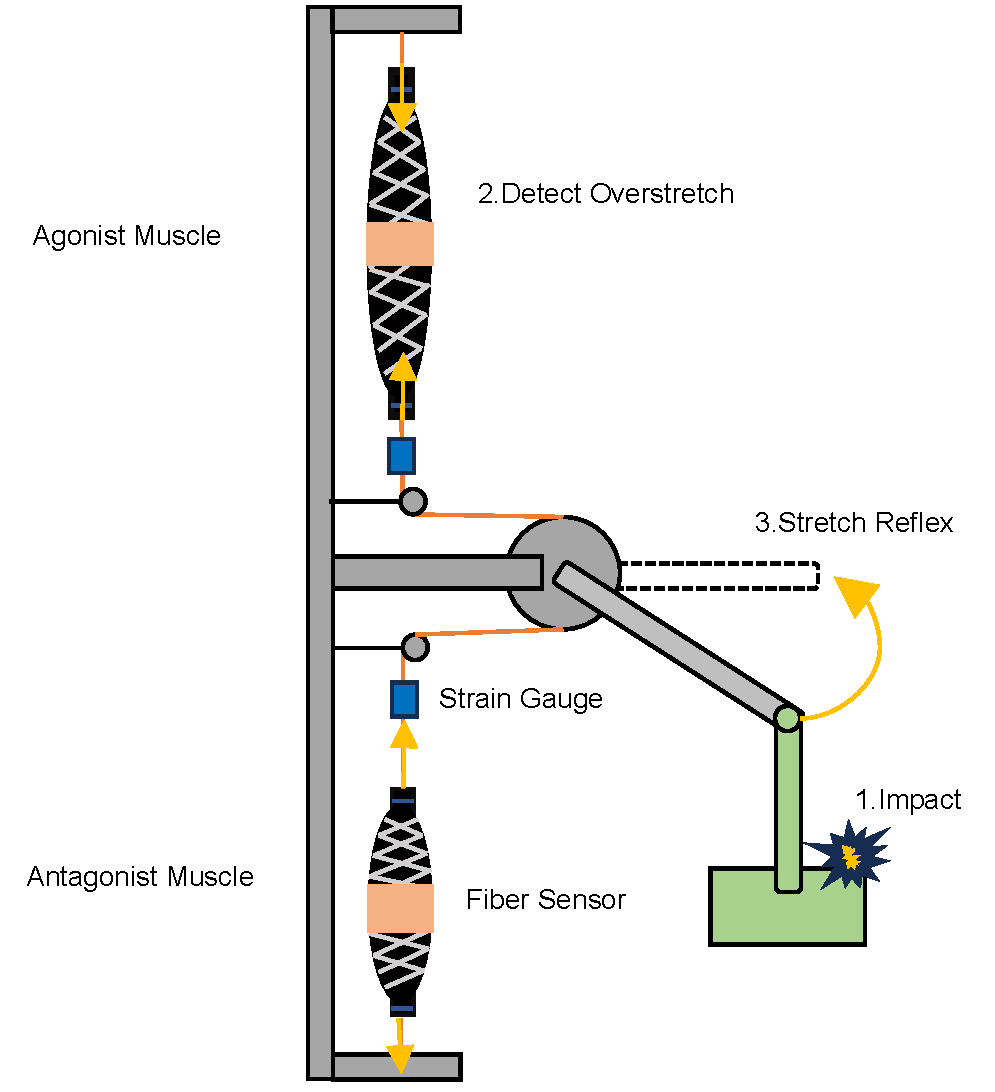
\includegraphics[width=0.7\columnwidth]{fig/reflex_experiment.pdf}
    \caption{Outline Diagram of Stretch Reflex Experiment}
    \label{fig:reflex_equipment}
 \end{figure}
Fig. \ref{fig:reflex_equipment} is an outline diagram of the stretch reflex experiment.
The arm was equipped with the basket and expected to keep it in a fixed position by maintaining the pressure of both PAMs at 0.4 $\si{MPa}$, and a 0.2 $\si{kg}$ mass was dropped from a height of 14 $\si{cm}$ to make an impact. During the experiment, the velocity of the PAMs was calculated as 
\begin{equation}
    \label{eq:velocity}
    v_j = \frac{l_j -l_{j-1}}{dt}
\end{equation}
where $j$ is the sampling number, $l_j$ is the estimated length, and $dt$ is the sampling period.
Since the system was set to 100 $\si{Hz}$, $dt$ was 0.01 $\si{s}$.
When the impact rapidly stretched the agonist PAM and its velocity exceeded a predetermined threshold, the stretch reflex was induced for 200 $\si{ms}$. The pressure command from the stretch reflex mechanism converged to the goal pressure from a top controller as follow:
\begin{align}
    \label{eq:command_pressure}
    p_{ago} &= p_{tp - ago} + \Delta p_{ago - exci} - \Delta p_{anta - inhi} \\
    p_{anta} &= p_{tp - anta} + \Delta p_{anta - exci} - \Delta p_{ago - inhi}
\end{align}
in which $p_{tp}$ is the goal pressure from the top controller,$\Delta p_{exci}$ is the excitatory pressure, and $ \Delta p_{inhi}$ is the reciprocal inhibition pressure. 
$\Delta p_{exci}$ and $\Delta p_{inhi}$ were calculated by the following equations:
\begin{equation}
    \label{eq:reflex_pressure}
    \Delta p_{exci} =  \Delta p_{inhi} = kv
\end{equation}
where $k$ is the gain determined experimentally.
Takahashi et al. designed this command process inspired by $\alpha$ motor neurons located in human spinal cords\cite{takahashi}. The positioning task was executed with stretch by the model and by the fiber sensor, and the reactions were compared.



%A foil strain gauge (KFP-5-120-C1-65L1M2R, Kyowa Electronic Instrument Co. Ltd) was glued to a 3mm aluminum board, and was attached to one end of each PAM. 
% Figure \ref{fig:dynamic_equipment} is an outline diagram of the experiment to verify the effectiveness of the proposed model by measuring the error when dynamically estimating the length of the PAMs using the acquired parameters. The experimental procedure is as follows: first, a weight of either $5\si{kg}$ or $10\si{kg}$ was connected to the PAMs via a pulley to apply a constant force $F$. Next, considering the strength of each PAM, the pressure $P [\si{MPa}]$ was 
% trigonometrically varied over time $t [\si{s}]$ by a proportional control valve (PCV) according to: sdads
% \begin{equation}
% P = 0.2 \sin\left(\frac{2 \pi t}{5}\right) + 0.6
% \label{eq:Pref}
% \end{equation}
% for PAM-A, PAM-B, and PAM-C, and:
% \begin{equation}
% P = 0.2 \sin\left(\frac{2 \pi t}{5}\right) + 0.4
% \label{eq:Prefd}
% \end{equation}
% for PAM-D. At each time, $F$, $P$, and the length $L$ of the PAMs were measured. 
% Finally, the errors were calculated between the measured and estimated $L$.

% \begin{figure}[h]
%     \centering
%     \includegraphics[width=\columnwidth]{fig/dynamic_experiment.pdf}
%     \caption{OUTLINE DIAGRAM OF THE DYNAMIC ESTIMATION EXPERIMENT}
% \label{fig:dynamic_equipment}
% \end{figure}


% \subsection{動的測定実験}
% 図\ref{fig:dnyamic_equipment}は,取得したパラメータを使用して動的に空気圧人工筋の長さを推定したときの
% 誤差を測定し,提案モデルの有効性を検証する実験の概略図である.実験の手順は次の通りである.
% まず,$5\si{kg}$もしくは$10\si{kg}$のウェイトをプーリーを介して空気圧人工筋に接続し,一定の張力をかけた.
% 次に,材料の強度を考慮して,比例制御弁により圧力$P[\si{MPa}]$を,
% PAM-A,PAM-B,PAM-Cに対しては,
% \begin{equation}
%   P =  0.2 \sin\left(\frac{2 \pi t}{5}\right) + 0.6 
% \label{eq:Pref}
% \end{equation}
% と,PAM-Dに対しては,
% \begin{equation}
%   P =  0.2 \sin\left(\frac{2 \pi t}{5}\right) + 0.4
% \label{eq:Prefd}
% \end{equation}
% と時間$t[\si{s}]$に対して動的に変化させ,各時刻の空気圧人工筋の全長$L$,張力$F$および圧力$P$の値を測定した.
% 最後に,全長$L$の推定値と測定値から誤差を計算した.





%\begin{table}[h]
%     \centering
%     \caption{The Characteristics of the experimented PAMs}
%     \begin{tabular}{c|ccccc}
%         \hline
%         空気圧人工筋 & 長さ [$\si{cm}$] & 直径 [$\si{mm}$] & 嚢構造の材料 \\
%         \hline \hline
%         PAM-A & 21.6 & 19.9 & 天然ゴム \\
%         PAM-B &21.1  & 13.4 & 天然ゴム \\
%         PAM-C & 14.1 & 13.4 & 天然ゴム \\
%         PAM-D & 21.2 & 19.0 & シリコン \\
%         \hline
%     \end{tabular}
%     \label{tab:PAM}
% \end{table}

% \begin{figure}[h]
%    \centering
%    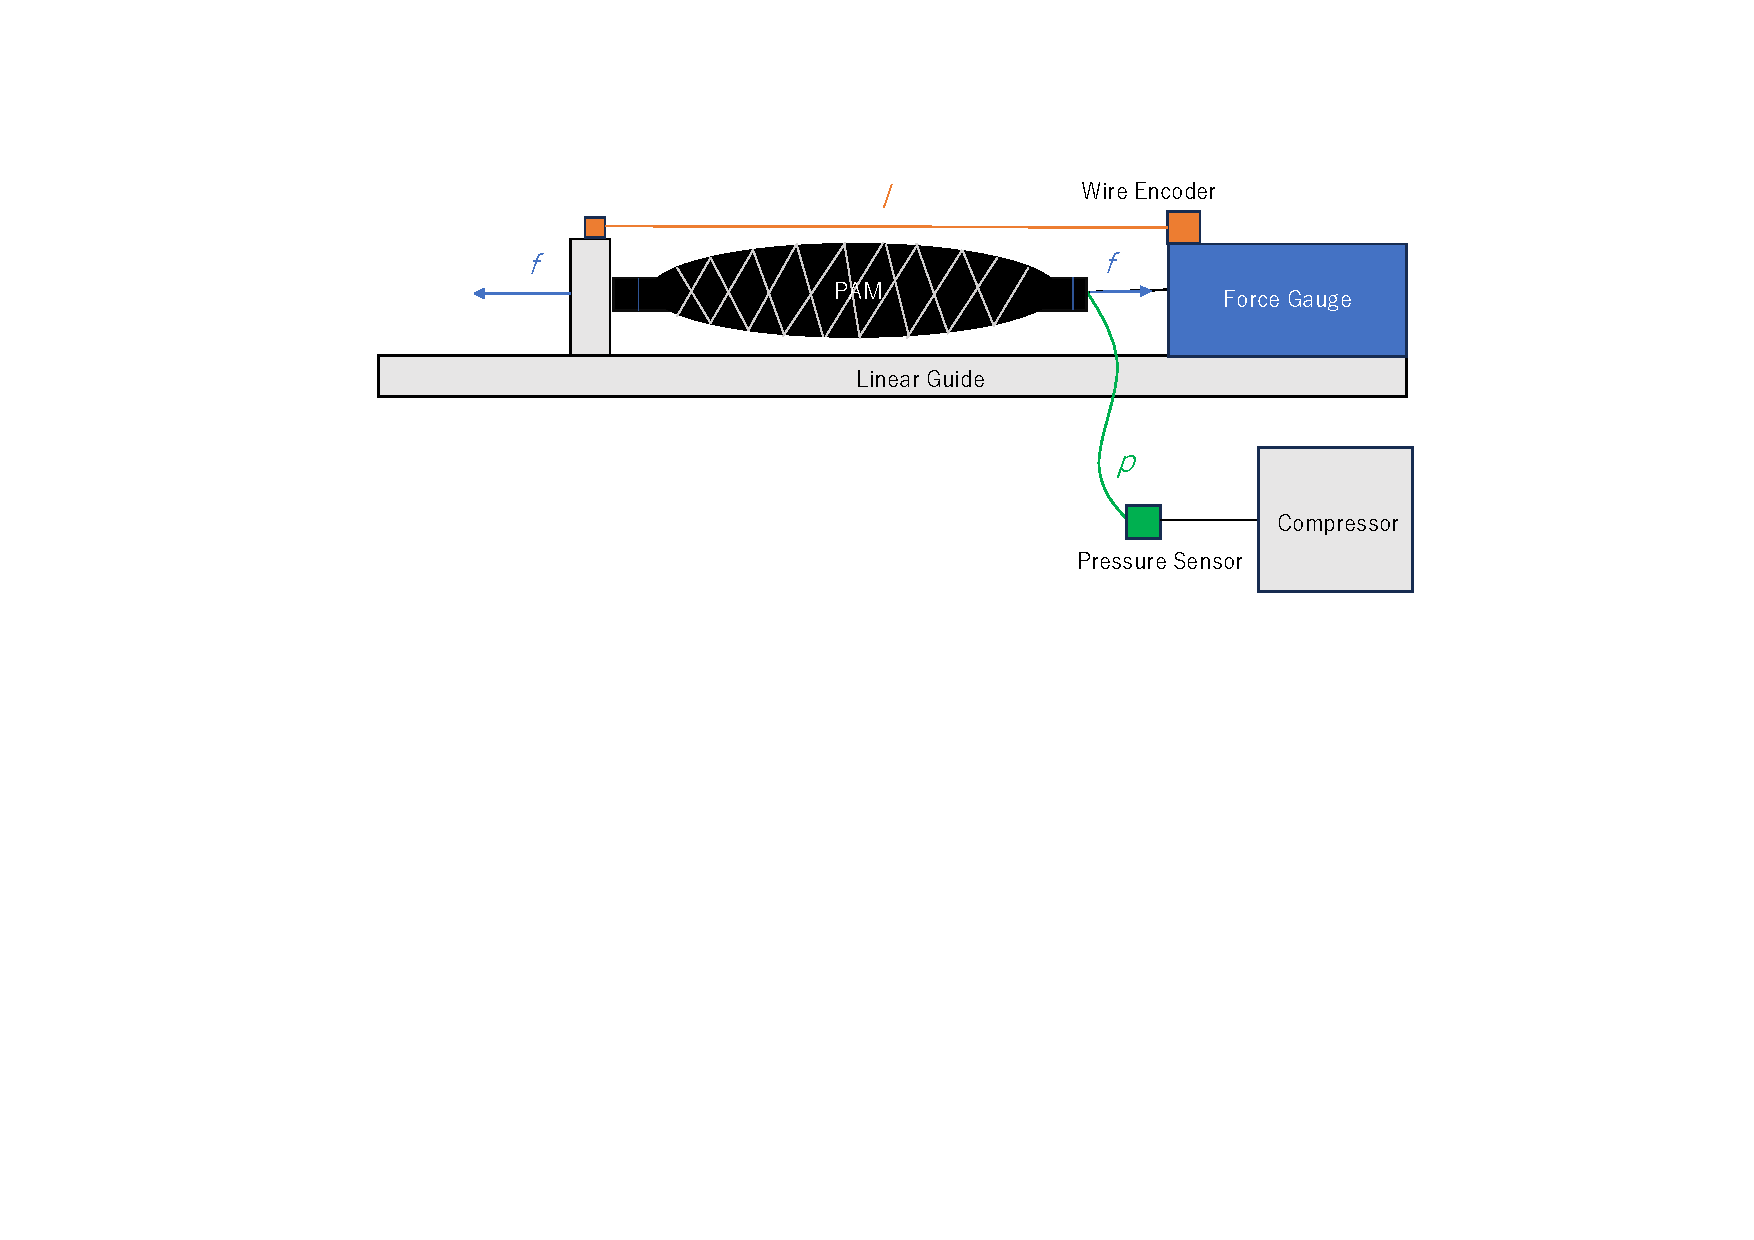
\includegraphics[width=\columnwidth]{fig/static_experiment.pdf}
%    \caption{Outline diagram of the parameter identification \\experiment}
%    \label{fig:static_equipment}
% \end{figure}

% \subsection{動的測定実験}
% 図\ref{fig:dnyamic_equipment}は,取得したパラメータを使用して動的に空気圧人工筋の長さを推定したときの
% 誤差を測定し,提案モデルの有効性を検証する実化の概略図である.実験の手順は次の通りである.
% まず,$5\si{kg}$もしくは$10\si{kg}$のウェイトをプーリーを介して空気圧人工筋に接続し,一定の張力をかけた.
% 次に,材料の強度を考慮して,比例制御弁により圧力$P[\si{MPa}]$を,
% PAM-A,PAM-B,PAM-Cに対しては,
% \begin{equation}
%   P =  0.2 \sin\left(\frac{2 \pi t}{5}\right) + 0.6 
% \label{eq:Pref}
% \end{equation}
% と,PAM-Dに対しては,
% \begin{equation}
%   P =  0.2 \sin\left(\frac{2 \pi t}{5}\right) + 0.4
% \label{eq:Prefd}
% \end{equation}
% と時間$t[\si{s}]$に対して動的に変化させ,各時刻の空気圧人工筋の全長$L$,張力$F$および圧力$P$の値を測定した.
% 最後に,全長$L$の推定値と測定値から誤差を計算した.

% \begin{figure}[h]
%    \centering
%    \includegraphics[width=\columnwidth]{fig/dynamic_experiment.pdf}
%    \caption{Outline diagram of the error measurement \\experiment}
%    \label{fig:dnyamic_equipment}
% \end{figure}

% 続いて,図1でPAMの左端を固定しているジグを外し,プーリーを設置した.また,圧力センサとコンプレッサの間に比例制御弁(PCV)を設置した.
% 5kgもしくは10kgのウェイトを空気圧人工筋に接続し,一定の張力$F$をかける負荷実験により,取得した推定パラメータの有効性を検証した.

